\chapter{Approach}
\label{Methods}

\section{Revisiting the Problem-Formulation}
A partitioning problem can be formally described as follows: Given a set of tables \textit{T} and queries \textit{Q}, for every table $T_i \in T$ with attributes $a_{i1},a_{i2},...,a_{in}$ we have to decide whether to replicate or to partition the table. For our approach, we only consider horizontal partitioning schemes using \textit{hash-partitioning}, which horizontally splits a table into a fixed number of shards (which is equal to the number of nodes in the database cluster). Thus, when two tables use the same partitioning attribute, we assume that they are co-partitioned on that attribute and equi-joins on that attribute do not involve any data-shuffling. For replication, we make a simplifying assumption: if a table is replicated, it is replicated to all nodes in the cluster. 
To summarise, in order to solve the partitioning problem, for each table, we thus have to decide whether that table is partitioned or replicated \cite{Hilprecht:2019:TLP:3329859.3329876}. If it is partitioned we additionally need to decide which attribute $a_i$ (or set of attributes) is being used for horizontal partitioning.
In their original work, \citeauthor{Hilprecht:2019:TLP:3329859.3329876}'s main intuition to model partitioning as a DRL problem was to model the database and the query workload as state and possible changes to the partitioning scheme as actions. In the following section, we first go through \citeauthor{Hilprecht:2019:TLP:3329859.3329876}'s version, and our proposed changes to the state-action pair.

\section{State}
A deep reinforcement learning neural network takes the state-action pair as input to the model to derive a Q-value for all possible actions, i.e. which partitioning or replicating actions to take. Therefore, it is quite fundamental to design the state in a manner that provides the model inference capabilities based on the state of the database cluster. In game playing learning scenarios such as teaching the agent how to play Atari \cite{DBLP:journals/corr/MnihKSGAWR13}, the state is encoded as the pixels of the game for any given frame. For such tasks, encoding the state is quite a straightforward approach, i.e. the pixels represent the state, $s_t$ at timestep $t$. In the case of a database partitioning task, \citeauthor{Hilprecht:2019:TLP:3329859.3329876} designs the state vector with the following considerations:

\subsection{Replication and Partition state}
For every table $T_i$, we have to encode whether it is currently partitioned or replicated. If it is partitioned, we additionally have to encode which attribute(s) are used for partitioning. Hence, for each table, we can encode its state as a binary vector using one-hot encoding:
\begin{equation}
    s(T_i) = (r_i, a_{i1},a_{i2},...,a_{in})
\end{equation}

\subsection{Workload Frequency}
The workload frequency for each query in the query workload $Q$ is also modelled as part of the state. For the same database schema, different workload frequencies would result in different optimal partitioning strategies that should be selected. For the purposes of this work, we assume that every possible query $q_i$ in a workload of queries $Q$ is known in advance. Given this scenario, the query workload can be represented as a vector where an entry encodes the frequency $f_i$ for a query $q_i$:
\begin{equation}
    s(Q) = (f_1,...,f_m)
\end{equation}
where $m$ is the total number of queries in the workload mix. The frequencies are normalised and hence, we obtain a vector where the entries are in the interval $[0,1]$. 

\subsection{Edges}
The concept of edges comes about in order to limit the search space and prevent sub-optimal partitioning schemes. As a result, we extend the state representation pushing the agent to explore only partitioning schemes where the tables are co-partitioned. To this end, every foreign key-primary key relationship between the attributes $a_{ir}$ and $a_{js}$ of the corresponding tables $T_i$ and $T_j$ includes an edge $(T_i,a_{ir},T_j,a_{js})$ which can either be active or inactive. If active, our approach guarantees that both relations are co-partitioned by that attribute if we perform a join between the two relations on that attribute, i.e. $T_i$ is hash-partitioned by $a_{ir}$ and $T_j$ is hash-partitioned by $a_{js}$. For example in Figure~\ref{fig:state-rep}, the edge $e_1$ is active and thus \texttt{lineorder} and \texttt{customer} table must be partitioned by the attributes \texttt{lo\_custkey} and \texttt{c\_custkey} respectively.



\begin{figure}[h]
  \centering
  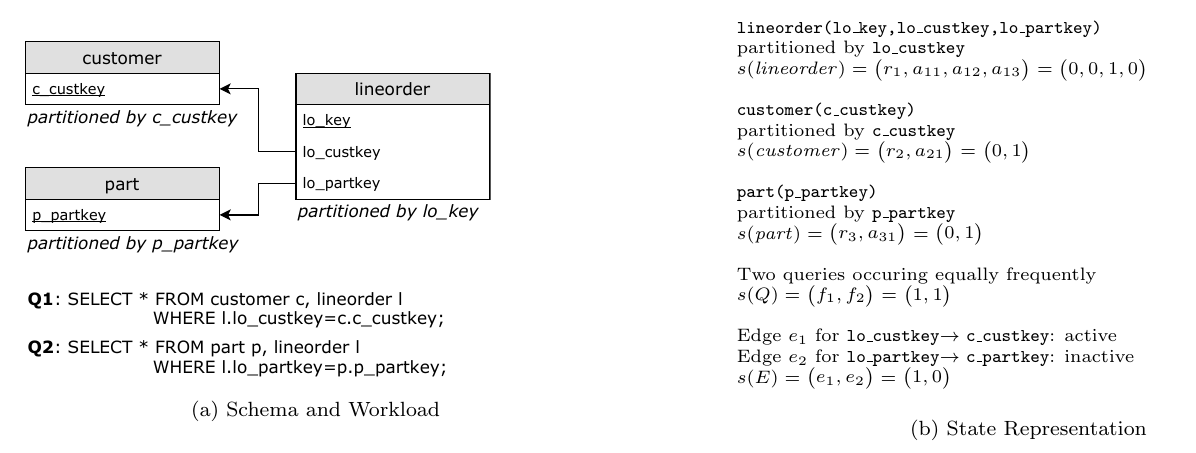
\includegraphics[width=\linewidth]{figures/simplified-ssb-schema-workload.png}
  \caption{Simplified SSB Schema and Workload}
  \label{fig:state-rep}

\end{figure}

\subsection{Modelling the Query and Query Optimiser as State}
\citeauthor{Hilprecht:2019:TLP:3329859.3329876} used the strategies discussed above in order to model the state for the DRL agent. However, there are a few limitations in the modelling above:
\begin{itemize}
    \item \textbf{Query Features} - Despite modelling the query workload frequencies as state, the rich features from the individual queries are not included in the state. 
    \item \textbf{Query Optimiser} - At no point is the cost information from the query optimiser used to model the state either. 
\end{itemize}

\subsection{Distributed Database - System X}
In order to fully understand the following methodology, we must first discuss the choice of the distributed database system - \textbf{System-X}. System-X is a pseudonym used for a commercial distributed database which supports SQL, \textbf{in-memory} rowstore tables and disk-backed columnstore tables. System-X was built specifically for horizontal-scale out architectures and its primary feature - in-memory rowstore design circumvents many of the issues that arise with disk-based databases. All of its functionality can be used through a MySQL wire protocol-compatible interface. The rowstore requires that all the data can fit in main memory. By completely avoiding disk IO, System-X makes use of a variety of techniques to speed up the execution, with minimal principal latencies. System-X supports two kinds of nodes in a cluster, i) \textbf{leaf} nodes store data and ii) \textbf{aggregator} nodes coordinate DML. One of the aggregator nodes is "master" and coordinates DDL. One of our major contribution is towards integrating System-X's query-optimiser as part of the DRL agent's state. Like most query-optimisers, System-X's query-optimiser generates plans for every query. But more importantly, System-X's query optimiser also provides insights about the distributed nature of the query alongside other key operations.

\subsection{Obtaining Query Optimiser Costs}
The cost information captures the cost of processing the query. However, a query usually has many possible physical plans and each plan has a different query cost. So it is not realistic to directly parse the query statement to extract the query cost. Instead, we generate query features using the query plan generated by the query optimiser, which has a cost estimate for each operation. System-X's query-optimiser generates the best plans for each query based on statistical analysis of the rows in each relation. The query plans also expose \textit{statistical row estimates} for key operations for each query. For example, consider the following scenario:

\begin{listing}[ht]
\inputminted[frame=lines,
            breaklines=true,
            framesep=2mm,
            fontsize=\footnotesize]
            {sql}
            {listings/query-optimiser-code.sql}
\caption{Example code to generate query-plan}
\label{listing:query-optimiser-code}
\end{listing}

Listing~\ref{listing:query-optimiser-code} generates the following query plan.

\begin{figure}[h]
  \centering
  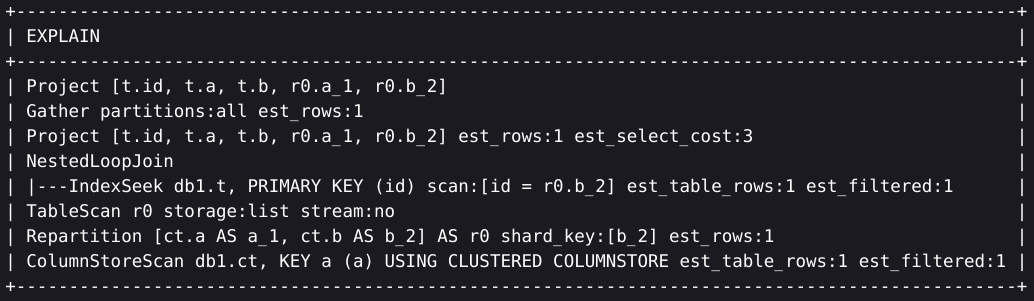
\includegraphics[width=\linewidth]{figures/explain-example.png}
  \caption{Example query plan generated for Listing~\ref{listing:query-optimiser-code}}
  \label{fig:explain-example}
\end{figure}

In total, System-X supports up to \textbf{17} operations. However, since our problem domain is the partitioning problem, not all operations are valuable to us. As such, we focus on the following operations:
\begin{itemize}
        \item Joins
        \begin{enumerate}
            \item \texttt{HashJoin} - performs a hash join: System-X builds a hash table from the results of the inner side of the join and probes into it while scanning the outer part of the join
            \item \texttt{MergeJoin} - performs a merge join: System-X scans both inner and outer sides of the join at the same time and merges matching rows
            \item \texttt{NestedLoopJoin} - performs a NestedLoop join: for every row on the outer side of the join System-X seeks or scans into the inner table to find all the matching rows
        \end{enumerate}
        \item Distributed Data Movement
        \begin{enumerate}
            \item \texttt{Gather} - collects all the results from the leaf nodes to the aggregator node. 
            \item \texttt{GatherMerge} - collects ordered streams of rows from the leaves and merges them to output an ordered stream
            \item \texttt{Repartition} - redistributes a dataset to hash-partition it on a particular key
            \item \texttt{Broadcast} - broadcasts a dataset to every node in a cluster
        \end{enumerate}
\end{itemize}
From this point, we will only be considering the \textit{estimated row counts} of the aforementioned operations. However, an astute observer might notice from Figure~\ref{fig:explain-example} that none of the join operations have any estimated row counts. A simple approach we took in order to calculate the cost of each join was by aggregating the total row count of each table access operation performed for each join. Consider the following query and its corresponding query plan, Figure~\ref{fig:tpc-ch-query-02-plan}.

\begin{listing}[ht]
\inputminted[frame=lines,
            breaklines=true,
            framesep=2mm,
            fontsize=\footnotesize]
            {sql}
            {listings/tpc_ch_02.sql}
\caption{TPC-CH Query 02}
\label{listing:tpc-ch-query-02}
\end{listing}

System-X supports 5 different kinds of table access methods, among which two are \texttt{ColumnStoreScan} and \texttt{OrderedColumnStoreScan}, both of which are only applicable for column-store tables. Since our approach only utilises row-store tables, we do not worry about the column-store based table access methods. As such, we only consider the following three table access methods:

\begin{itemize}
    \item \texttt{TableScan} - scans every row in a table using an index
    \item \texttt{IndexSeek} - navigates to a particular row using an index
    \item \texttt{IndexRangeScan} - scans a range of rows using an index
\end{itemize}

\begin{figure}[h]
  \centering
  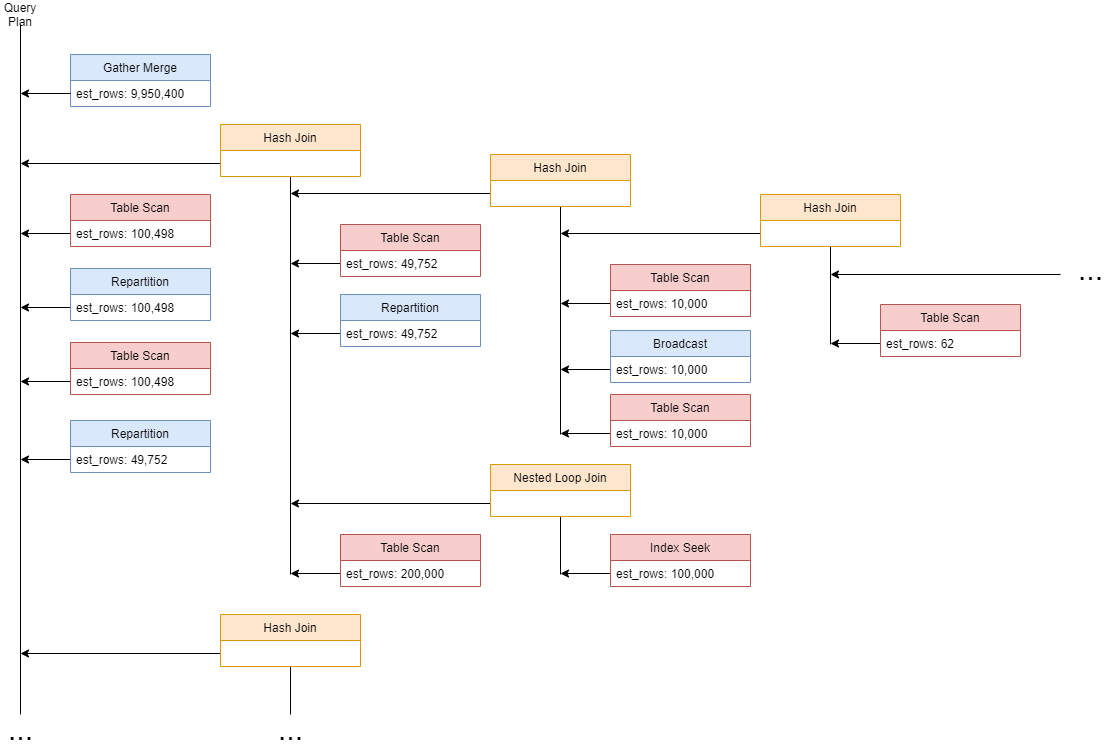
\includegraphics[width=\linewidth]{figures/query_02_plan_01.png}
  \caption{A section of the query plan for Listing~\ref{listing:tpc-ch-query-02}}
  \label{fig:tpc-ch-query-02-plan}
\end{figure}

In Figure~\ref{fig:tpc-ch-query-02-plan}, table access operations are illustrated in red, join operations in yellow and all other operations in blue. The rest of the diagrams will remain thematically consistent with this approach. Once we calculate the join costs, the query plan could be illustrated as in Figure~\ref{fig:join-cost-calculation}.

\begin{figure}[h]
  \centering
  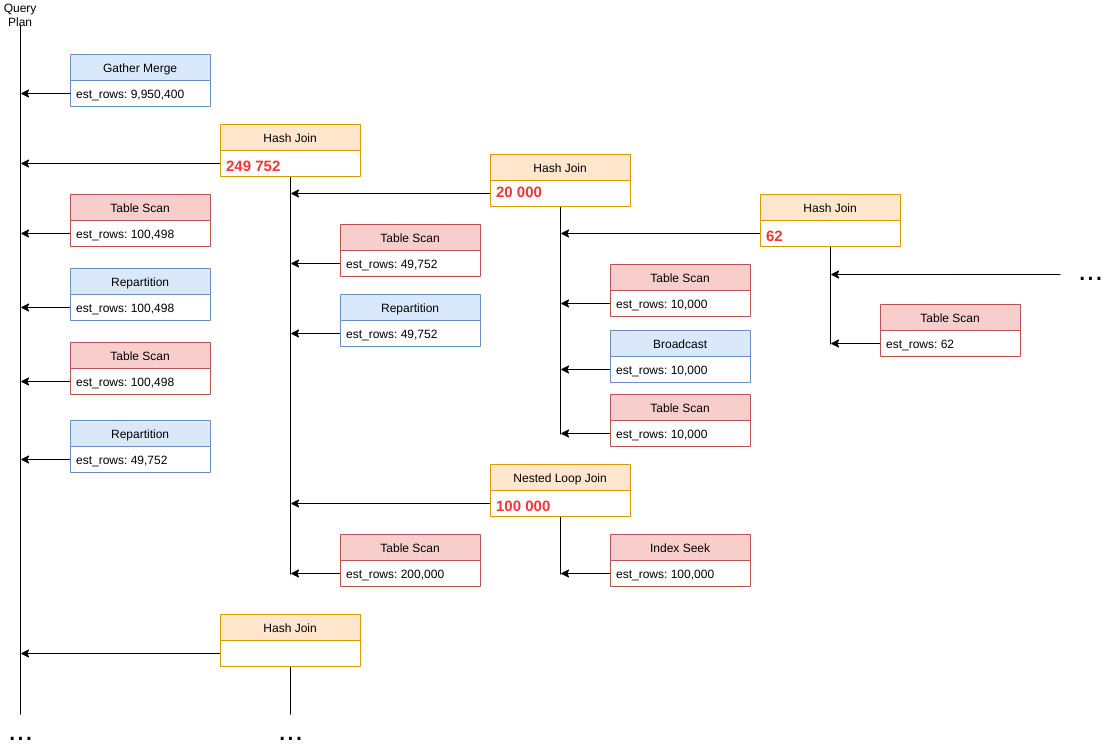
\includegraphics[width=\linewidth]{figures/query_02_plan_02.png}
  \caption{Join cost calculation for TPC-CH Query 02}
  \label{fig:join-cost-calculation}
\end{figure}


\subsection{Intuition for Query Optimiser and Query Featurisation}
However, before we explain how the query optimiser and query features are integrated into the model, let's try to understand the intuition behind why integrating the state of the query workload and the optimiser could be beneficial. Consider the following query, which is the 5th query from the TPC-CH benchmark.

\begin{listing}[ht]
\inputminted[frame=lines,
            breaklines=true,
            framesep=2mm,
            fontsize=\footnotesize]
            {sql}
            {listings/tpc_ch_05.sql}
\caption{TPC-CH Query 05}
\label{listing:tpc-ch-query-05}
\end{listing}

This query can be used to highlight how different partitioning schemes can give rise to different optimal query plans. For example, this query requires multiple equi-joins between several relations on several attributes, such as:
    \begin{itemize}
        \item \texttt{c\_id = o\_c\_id}
        \item \texttt{ol\_o\_id = o\_id}
        \item \texttt{ol\_i\_id = s\_i\_id}
    \end{itemize}
From the perspective of a database administrator, if we were to try to optimise this query for performance, we would like for the two biggest relations, in this case \texttt{orders} and \texttt{orderline} to be co-partitioned. Given that we would like to optimise this query, we could come up with the following partitioning scheme:
    \begin{itemize}
        \item orderline \texttt{SHARD KEY (ol\_o\_id, ol\_w\_id, ol\_d\_id)}
        \item orders \texttt{SHARD KEY (o\_id, o\_w\_id, o\_d\_id)}
        \item enable local reference joins between the two largest relations and reduce re-partitioning costs.
        \item consider a partitioning scheme where all tables are replicated except for \texttt{orderline} and \texttt{orders} which are co-partitioned.
    \end{itemize}

The complete plan generated by query-05 from Listing~\ref{listing:tpc-ch-query-05} can be found in    

\section{Compound Key Partitioning Actions}

\subsection{Time Complexity}

\section{Query Featurisation}

\subsection{Topological Modelling of the DRL agent}

\subsection{Statistics-driven approach}
